\documentclass{article}

\usepackage[dblblindworkshop, final]{template/neurips_2026}
\workshoptitle{Sim2Science: ML with Imperfect Scientific Models}

\usepackage[utf8]{inputenc}
\usepackage[T1]{fontenc}
\usepackage{hyperref}
\usepackage{url}
\usepackage{booktabs}
\usepackage{amsfonts}
\usepackage{amsmath}
\usepackage{microtype}
\usepackage{graphicx}
\usepackage{xcolor}

% Camera-ready: the template's float, caption and display spacing is used unchanged.

% Working-draft macros -----------------------------------------------------
\newcommand{\todo}[1]{\textcolor{red}{[TODO: #1]}}
% Release repository (verify the public URL at publication).
\newcommand{\repourl}{https://github.com/covinolab/short-simulators-long-experiments}
\newcommand{\fD}{f_{\mathrm{D}}}
\newcommand{\DA}{D_{\mathrm{A}}}
\newcommand{\koff}{\kappa_{\mathrm{OFF}}}
\newcommand{\pp}{\,\mathrm{pp}}

\title{Short Simulators, Long Experiments: A Controlled Audit of Horizon
Mismatch in Simulation-Based Inference for Live-Cell Microscopy}

\author{%
  Michael Alexander Ramirez Sierra \quad Roberto Covino\\
  Goethe University Frankfurt, Faculty of Mathematics and Computer Science\\
  Cluster of Excellence SubCellular Architecture of Life (SCALE)\\
  Frankfurt Institute for Advanced Studies (FIAS), Frankfurt am Main, Germany\\
  \texttt{ramirez-sierra@fias.uni-frankfurt.de} \quad \texttt{covino@fias.uni-frankfurt.de}\\
}

\begin{document}

\maketitle

\begin{abstract}
Amortized simulation-based inference (SBI) may be trained on short synthetic
recordings and then applied to consecutive windows of longer experiments.
Unlike independent training clips, later windows inherit molecular
composition, spatial correlations, and photophysical history. We quantify
this horizon mismatch in a reaction--diffusion model of receptor dimerization
with synthetic live-cell microscopy. For each of 500 parameter settings, we
compare ten independent 2\,s simulations with ten consecutive 2\,s windows
from one 20\,s simulation, using exact simulator truth. We examine the
dimer-complex fraction, dimer unbinding rate, and monomer diffusion
coefficient. By the final window, errors in the first two exceed prespecified
tolerances, whereas diffusion remains within tolerance. For dimer
composition, 90\% interval coverage falls from 0.95 to 0.39 without wider
posterior intervals. Averaging windows reduces total error but not the
history-induced error. We use its simulated magnitude as a sensitivity test,
not a correction, for experimental MET recordings. The difference between
resting and activated conditions remains much larger than this effect.
However, absolute fractions remain model-dependent, and the workflow does not
support interpreting a whole-recording unbinding estimate as a single
constant rate. Short-window SBI should therefore be validated separately for
each inferred quantity and aggregation rule.
\end{abstract}

\section{Introduction}
\label{sec:intro}

Simulation-based inference (SBI) trains a neural estimator on forward
simulations and applies it to observations
\citep{cranmer2020frontier,greenberg2019automatic,boelts2025sbi}.
Its validity therefore depends not only on the simulator's physics, but also
on whether the training simulations represent the inputs encountered during
deployment.

Short clips are the practical training unit: amortized training needs a
large corpus of simulated videos, and clip length sets the cost of
simulating, rendering, and training on each one. Experimental recordings are
longer because the temporal evolution they contain is itself of interest, so
a recording is analyzed through consecutive windows of training length. In the audit, the continuous simulation starts from the training
initialization distribution, and later windows inherit changes in molecular
populations, spatial correlations, and photophysical state from the
preceding dynamics (Fig.~\ref{fig:design}). We call this difference the \emph{horizon mismatch}
and the assumption that it does not affect inference the \emph{reset
assumption}. It is one form of deployment mismatch: the states and histories
presented to the estimator differ from those represented in training, even
though the simulator itself is unchanged. Both audit arms share the same
parameters, dynamics, imaging model, and prior, and every window or clip is a
2\,s input to the same estimator; the arms differ only in whether each window
is initialized independently or inherits the history of a continuous
trajectory.

\begin{figure}[t]
\centering
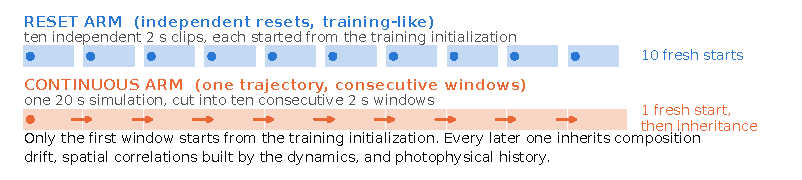
\includegraphics[width=\linewidth]{figures/fig1_design}
\caption{\textbf{Testing the reset assumption.} Training uses independently
initialized 2\,s clips. In the continuous audit simulation, one 20\,s trajectory is divided into
ten consecutive windows, of which only the first begins from the training
initialization distribution. $(A_0,B_0,C_0)$ are the initial
counts of free monomeric receptors, mobile dimers, and immobilized dimers.
The composition truth for each window is its exact first-frame population;
a matched reset clip starts again from $(A_0,B_0,C_0)$.}
\label{fig:design}
\end{figure}

That finite-time statistics depend on initialization and history is well
established for stochastic processes, including aging and non-ergodic systems
\citep{metzler2014anomalous}, but this does not determine how a trained
neural estimator responds to such history. Studies of SBI robustness have
examined perturbed observations, discrepancy models, incompatible summaries,
and test-time distribution shifts
\citep{cannon2022investigating,ward2022robust,frazier2021synthetic,schmitt2023detecting},
and calibration diagnostics assess an estimator relative to a specified
simulator distribution \citep{talts2018validating,lemos2023sampling}; if
held-out simulations repeat the reset initialization used for training, they
cannot reveal errors caused by inherited state.

Compositional SBI for time series addresses long sequences by learning
single-state transitions from a proposal intended to cover the reachable
state space \citep{gloeckler2025compositional}. We ask the complementary
question: how accurately does an already-trained short-window estimator
operate when applied unchanged along a continuous trajectory? In
single-molecule applications, simulator mismatch is recognized as an
important limitation \citep{dingeldein2025simulation}, but existing
benchmarks evaluate independently simulated trajectories or fixed-duration
fields of view
\citep{munozgil2021objective,munozgil2025quantitative}. DeepSPT combines a
simulation-trained segmentation module with classifiers trained on annotated
experimental data \citep{kaestelhansen2025deep}. Among these studies, none
reports a controlled reset-versus-continuous comparison with known
window-specific truth.

We contribute a paired reset-versus-continuous audit with exact simulator
truth and prespecified operational tolerances \citep{lakens2018equivalence};
evidence that horizon mismatch affects composition, kinetics, and diffusion
differently within one single-particle-tracking inference workflow; and the
use of the measured horizon-mismatch error as a sensitivity test, not a
correction, for the workflow's conclusions from experimental MET recordings.

\section{System: simulator, estimator, and deployment}
\label{sec:system}

\paragraph{Simulator.} We represent membrane-receptor dimerization as the
particle-based reaction--diffusion process
$A + A \rightleftharpoons B \rightleftharpoons C$, where $A$ is a freely
diffusing monomeric receptor, $B$ a mobile dimer, and $C$ an immobilized
dimer represented as an effective state. Simulations use ReaDDy
\citep{hoffmann2019readdy} and follow earlier amortized-inference work on
spatial-stochastic biological systems \citep{ramirezsierra2025sgm}. The ten
parameters have log-uniform priors and comprise the initial counts of
$A$, $B$, and $C$; the monomer diffusion coefficient $\DA$
($\mu\mathrm{m}^2\,\mathrm{s}^{-1}$); two relative-mobility ratios; an
association-efficiency parameter $R_{\mathrm{ON}}$, defined relative to the
diffusion-limited association ceiling; and the rates of dimer unbinding ($\koff$), immobilization, and
remobilization ($\mathrm{s}^{-1}$). Particle trajectories are rendered as synthetic
videos using a fixed, experiment-informed microscopy model.

\paragraph{Estimator.} Each 2\,s input contains 100 video frames. A
five-block three-dimensional convolutional network extracts local
spatiotemporal features, and a two-layer temporal Transformer integrates
them across the clip into a 128-dimensional representation
\citep{vaswani2017attention}. This representation conditions a masked
autoregressive flow that approximates the joint posterior over the ten model
parameters \citep{papamakarios2017masked}. The estimator is trained by neural
posterior estimation \citep{greenberg2019automatic} using the \texttt{sbi}
toolkit \citep{boelts2025sbi}.

For each window we draw 1,000 joint posterior samples; directly inferred
parameters are summarized by their marginal posterior medians. The
\emph{dimer-complex fraction}, $\fD=(B+C)/(A+B+C)$, the fraction of simulated
molecular complexes that are dimers, is calculated within every joint draw,
preserving dependence among the three counts, and summarized by its
posterior mean and central 90\% interval. On 10,000 independently generated held-out videos, the mean
absolute error is $2.8$ percentage points for $\fD$. For $\DA$ and $\koff$,
the log-scale mean absolute errors correspond to multiplicative factors of
$\times1.05$ and $\times1.50$, respectively. The association-efficiency
parameter $R_{\mathrm{ON}}$ is not identifiable from the tested 2\,s videos,
so no subsequent scientific claim is based on it. Training and data-split
details are given in Appendix~\ref{app:training}.

\paragraph{Experimental deployment.} MET is a receptor tyrosine kinase of
the plasma membrane; binding of its ligands, including the bacterial protein
InlB, is associated with receptor dimerization and signaling. Single-particle
tracking follows individually labeled receptors in living cells. We apply
the estimator directly to MET recordings acquired for single-particle tracking
\citep{harwardt2017membrane}: 25 recordings of resting MET labeled with a
non-activating Fab fragment and 25 recordings of MET labeled and activated by
fluorescent InlB. Independent single-molecule studies report increased MET
dimerization after ligand binding \citep{dietz2013single,baldering2021crispr},
which supports describing the InlB condition as dimerization-enriched but
provides no stoichiometric ground truth for these recordings.

Each 20\,s recording is divided into ten consecutive 2\,s windows, matching
the estimator's training duration. The estimator produces one result per
window; the ten results are averaged to one value per cell, the independent
biological replicate, so horizon mismatch is evaluated at both the window and
the recording level.

\section{The horizon audit}
\label{sec:design}

\paragraph{Design.} For every parameter setting, we generate two matched
audit arms with identical parameters and imaging. The \emph{continuous} arm
is one 20\,s simulation divided into ten consecutive 2\,s windows. The \emph{reset} arm contains ten independently initialized 2\,s simulations.
Every window and every clip is a 2\,s input to the fixed estimator used for
the experimental recordings, so the arms differ in initialization and
inherited history, not in input length. Two of 502 attempted settings were rejected, leaving 500
(disposition, seeding, and cohort tracking in Appendix~\ref{app:truthref}).

\paragraph{Truth reference.} The simulator stores the exact $A$, $B$, and
$C$ populations at every frame of the rendered trajectory, so the composition
truth belongs to the same stochastic realization as the estimator input and is
not reconstructed from the image. Training
labels represent the population at the beginning of a clip, so the primary
truth for window $j$ is its exact first-frame population, from which $\fD$ is
calculated. At the recording level, we average both the ten inferred values
and the ten window-start truths. Alternative truth definitions are examined
in Appendix~\ref{app:truthref}.

\paragraph{Statistics.} Each matched parameter setting is one independent
statistical unit; the ten windows from its continuous trajectory are
correlated repeated measurements
\citep{lazic2010pseudoreplication}. We calculate 95\% percentile confidence
intervals from 2,000 bootstrap resamples of the 500 settings. For setting
$i$ and window $j$, the primary statistic is the difference between the
continuous-window absolute error and the mean absolute error of the ten
matched reset clips:
%
\begin{equation}
\Delta_{ij}
= \bigl|\hat y^{\,\mathrm{cont}}_{ij} - y^{\star}_{ij}\bigr|
- \frac{1}{R}\sum_{r=1}^{R}
  \bigl|\hat y^{\,\mathrm{reset}}_{ir} - y^{\star}_{ir}\bigr|,
\qquad R=10.
\label{eq:delta}
\end{equation}
%
Positive values indicate lower accuracy in the continuous arm. For constant
parameters, $y^{\star}_{ij}=\theta^{\star}_{i}$; for $\fD$, the truth changes
with the window-start population. The analogous contrast without absolute
values is called the \emph{signed shift} and describes the direction of the
inference error.

The three primary quantities were declared before the audit: the
dimer-complex fraction $\fD$, dimer unbinding rate $\koff$, and monomer
diffusion coefficient $\DA$. Individual species counts and the remaining
parameters are treated as exploratory diagnostics. Each primary quantity has
a prespecified tolerance equal to its mean absolute error on independently
initialized held-out videos. This estimator-relative operational tolerance, not a biological effect-size
threshold, asks whether horizon mismatch adds at least as much error as the
estimator already carries under its validation conditions.

Following equivalence-testing logic \citep{lakens2018equivalence}, a quantity
is \emph{degraded} when its entire confidence interval lies above the
positive tolerance, \emph{equivalent} when the interval lies within the
negative and positive tolerance bounds, and \emph{inconclusive} otherwise.
Comparison with zero alone establishes detectability, not whether the
additional error is large relative to baseline performance. Before
interpreting later windows, the prespecified first-window gate requires all
three primary quantities to be equivalent within their respective
tolerances.

\section{Results}
\label{sec:results}

\begin{figure}[t]
\centering
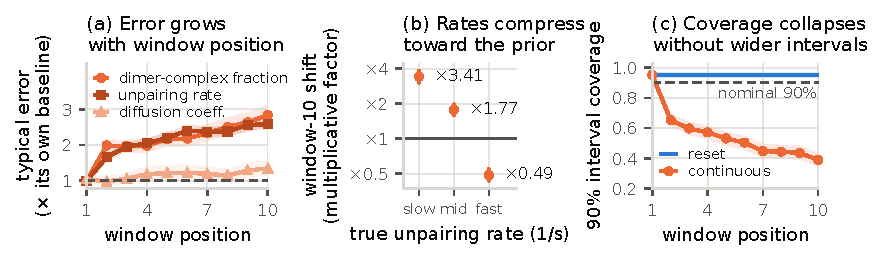
\includegraphics[width=\linewidth]{figures/fig2_result}
\caption{\textbf{Horizon mismatch affects the three quantities differently.}
(a) Mean absolute error by window position, divided by each quantity's
held-out error (dashed line). Composition and unbinding-rate errors approach
three times their baselines, whereas diffusion changes modestly. Verdicts
use the matched horizon contrast in Table~\ref{tab:headline}. (b) Signed
unbinding-rate shift at window 10 by true-rate third: slow rates are read
high and fast rates low, indicating compression toward the prior interior.
(c) Coverage of the central 90\% interval
for $\fD$. Coverage in the continuous arm falls to $0.39$ without wider
intervals. Bands and bars are 95\% bootstrap intervals over matched
settings.}
\label{fig:result}
\end{figure}

\subsection{Horizon mismatch affects the primary quantities selectively}
\label{sec:headline}

At window 1, every continuous-minus-reset confidence interval lies within
its prespecified tolerance: $+0.00\pp$ $[-0.22,+0.22]$ for $\fD$,
$\times1.00$--$\times1.01$ for $\DA$, and
$\times0.97$--$\times1.03$ for $\koff$. The first-window gate therefore
passes: the arms are comparable before recording history accumulates.

By window 10, the dimer-complex fraction and unbinding-rate errors exceed
their tolerances, whereas the diffusion-coefficient error remains within
tolerance (Table~\ref{tab:headline}). Averaging the ten windows reduces total
error but leaves all three verdicts unchanged, so the horizon-dependent error
persists at the recording level.

\begin{table}[t]
\caption{Results over 500 matched parameter settings. Total error is the
mean absolute error; the horizon contrast is continuous minus reset absolute
error, expressed for the log-scale parameters as a ratio of error factors
($\times1$: no additional error). Verdicts compare the entire 95\% confidence
interval with the tolerance; recording-level values average ten windows under
the same tolerances.}
\label{tab:headline}
\centering
\footnotesize
\begin{tabular}{lcccc}
\toprule
quantity, level & total error (reset $\rightarrow$ cont.) & horizon contrast [95\% CI] & tolerance & verdict \\
\midrule
$\fD$, window 10 & $2.9\rightarrow8.3\pp$ & $+5.4\ [4.7,6.2]\pp$ & $2.8\pp$ & degraded \\
$\fD$, recording & $1.7\rightarrow5.6\pp$ & $+3.9\ [3.4,4.4]\pp$ & $2.8\pp$ & degraded \\
$\koff$, window 10 & $\times1.53\rightarrow\times3.02$ & $\times1.97\ [1.85,2.10]$ & $\times1.50$ & degraded \\
$\koff$, recording & $\times1.38\rightarrow\times2.22$ & $\times1.61\ [1.55,1.68]$ & $\times1.50$ & degraded \\
$\DA$, window 10 & $\times1.05\rightarrow\times1.07$ & $\times1.02\ [1.01,1.03]$ & $\times1.05$ & equivalent \\
$\DA$, recording & $\times1.03\rightarrow\times1.05$ & $\times1.01\ [1.01,1.02]$ & $\times1.05$ & equivalent \\
\bottomrule
\end{tabular}
\end{table}

For $\fD$, lower accuracy is not accompanied by greater posterior
uncertainty: the central 90\% intervals cover the truth in $95\%$ of settings
at window 1 but only $39\%$ at window 10 while their widths do not grow
(Appendix~\ref{app:truthref}), so posterior width alone does not reveal this
mismatch. The degradation also
persists when populations remain within the training initialization range,
so range escape alone does not explain it (Appendix~\ref{app:support}).

\subsection{Unbinding-rate estimates shift toward the training-range interior}
\label{sec:structure}

Because held-out accuracy varies with the true value, we repeated the
analysis in prespecified parameter strata with local tolerances
(Appendix~\ref{app:strata}). Composition is degraded in both
adequately sampled strata; the highest-composition stratum contains only two
settings and is not assessed. The unbinding rate is degraded in the slow and
fast thirds and inconclusive in the middle. For $\DA$, the lowest third is
equivalent and the remaining two are inconclusive; none is degraded.

The signed $\koff$ shift decreases monotonically with the true rate
(Fig.~\ref{fig:result}b). Relative to the matched reset arm, window-10
estimates are shifted by factors of $\times3.41$, $\times1.77$, and
$\times0.49$ across the slow, intermediate, and fast thirds. Thus, slow
rates are estimated too high and fast rates too low, compressing estimates
toward the prior interior. This pattern is consistent with reduced
information about the true rate, although the audit does not identify the
estimator-level cause (Appendix~\ref{app:mechanism}). The compression remains after recording-level
aggregation.

\subsection{Sensitivity of conclusions from experimental MET recordings}
\label{sec:census}
\label{sec:claims}

For the MET recordings, the estimator reports the relative abundance of
simulated complex categories, not molecular stoichiometry. The inferred
dimer-complex fraction is $31.4\pm2.0\%$ for resting MET-FAB and
$78.2\pm3.7\%$ for activated MET-INLB (mean $\pm$ s.e.m.,
$n=25$ cells per condition). The cell-level distributions differ in a
Mann--Whitney U test ($p\approx2\times10^{-9}$). Within MET-INLB recordings,
the mean decreases from $87.0\%$ in the first window to $70.2\%$ in the last
(paired Wilcoxon test, $p=0.0015$).

We use the simulated recording-level shifts as an uncalibrated sensitivity
scale for the experimental conclusions (transfer rules and absolute values in
Appendices~\ref{app:verdicts} and~\ref{app:census}), not as corrections or
uncertainty bounds.

\emph{The condition contrast remains supported under direct transfer.}
The difference between MET-FAB and MET-INLB changes from $46.8\pp$ to about
$48.3\pp$ (Fig.~\ref{fig:census}, with the inferred time courses); the
simulated horizon effect is therefore too small to generate the observed
condition difference.

\emph{The horizon effect does not generate the within-recording decline.}
Inherited history shifts late-window $\fD$ upward in simulation, opposite to
the observed $87.0\%\rightarrow70.2\%$ decrease; it would therefore mask part
of the decline rather than create it.

\emph{Absolute composition and unbinding-rate estimates remain conditional.}
The transfers establish relative scale only; they neither correct the
experimental estimates nor identify the cause of their temporal trends.

\section{Discussion and conclusions}
\label{sec:discussion}

\paragraph{Reliability is quantity-specific.} Because the arms pass the
first-window gate, later degradation is caused by what later windows inherit,
not by clip duration alone. Under the tested mismatch, $\DA$ remains within
tolerance, whereas $\fD$ loses accuracy and interval coverage, and averaging
does not remove the additional error. The unbinding-rate error is larger and
rate-dependent, with slow rates shifted upward and fast rates downward, so a
whole-recording estimate cannot be interpreted as one constant unbinding
rate. For the MET recordings, direct transfer is too small to explain the
condition contrast, although absolute fractions remain conditional.

\paragraph{Scope and implication.} This audit isolates a reset-trained
estimator applied to history-inheriting windows within one model; it neither
tests other misspecification nor explains experimental trends, distinguishes
mechanisms, or provides a correction. Since held-out reset clips cannot establish performance after stateful
evolution, validation should reproduce the deployed inference sequence, use
the trajectory as the statistical unit, and evaluate each reported quantity
and aggregation rule against simulator truth; training can instead use
full-length simulations or clips from reachable states. Reliability must be
established per conclusion, not for the estimator as a whole.

% Line numbers exist only in the anonymized build; the final option loads no lineno.
\makeatletter\@ifundefined{nolinenumbers}{}{\nolinenumbers}\makeatother
% Acknowledgments (template ack environment, shown only in the final build) go here,
% after the main text and before the references, outside the reduced-font group below.
\begin{ack}
We thank all members of Roberto Covino's Computational Life Science Lab for
helpful discussions. We acknowledge the support of Goethe University Frankfurt
and the Frankfurt Institute for Advanced Studies (FIAS). This work was
supported by the Cluster of Excellence SubCellular Architecture of Life
(SCALE).
\end{ack}

% The reduced font size applies to the references only.
\begingroup
\small
\bibliographystyle{plainnat}
\bibliography{references}
\endgroup

\newpage
\section*{NeurIPS Paper Checklist}




\begin{enumerate}

\item {\bf Claims}
    \item[] Question: Do the main claims made in the abstract and introduction accurately reflect the paper's contributions and scope?
    \item[] Answer: \answerYes{} % Replace by \answerYes{}, \answerNo{}, or \answerNA{}.
    \item[] Justification: The abstract and introduction state the horizon mismatch, the controlled audit, its selective outcome across the three primary estimands, and the claim-specific sensitivity analysis. Sections 4.1--4.3 provide the supporting results. Scope limits (in-simulator audit, one system, one estimator, and uncalibrated simulator-to-experiment transfer) are stated in the abstract and Section 5.
    \item[] Guidelines:
    \begin{itemize}
        \item The answer \answerNA{} means that the abstract and introduction do not include the claims made in the paper.
        \item The abstract and/or introduction should clearly state the claims made, including the contributions made in the paper and important assumptions and limitations. A \answerNo{} or \answerNA{} answer to this question will not be perceived well by the reviewers. 
        \item The claims made should match theoretical and experimental results, and reflect how much the results can be expected to generalize to other settings. 
        \item It is fine to include aspirational goals as motivation as long as it is clear that these goals are not attained by the paper. 
    \end{itemize}

\item {\bf Limitations}
    \item[] Question: Does the paper discuss the limitations of the work performed by the authors?
    \item[] Answer: \answerYes{} % Replace by \answerYes{}, \answerNo{}, or \answerNA{}.
    \item[] Justification: Section 5 states that the audit measures the cost of the reset assumption inside the simulator only, does not identify the cause of the drift observed in experimental data, and rests on one system and one estimator. Appendix C presents the candidate mechanisms as hypotheses and states that the two proposed controlled ablations have not been executed. Section 4.3 states that simulator-to-experiment transfer is uncalibrated, so the simulated horizon effect is used only as a sensitivity scale and never as a correction to the experimental values.
    \item[] Guidelines:
    \begin{itemize}
        \item The answer \answerNA{} means that the paper has no limitation while the answer \answerNo{} means that the paper has limitations, but those are not discussed in the paper. 
        \item The authors are encouraged to create a separate ``Limitations'' section in their paper.
        \item The paper should point out any strong assumptions and how robust the results are to violations of these assumptions (e.g., independence assumptions, noiseless settings, model well-specification, asymptotic approximations only holding locally). The authors should reflect on how these assumptions might be violated in practice and what the implications would be.
        \item The authors should reflect on the scope of the claims made, e.g., if the approach was only tested on a few datasets or with a few runs. In general, empirical results often depend on implicit assumptions, which should be articulated.
        \item The authors should reflect on the factors that influence the performance of the approach. For example, a facial recognition algorithm may perform poorly when image resolution is low or images are taken in low lighting. Or a speech-to-text system might not be used reliably to provide closed captions for online lectures because it fails to handle technical jargon.
        \item The authors should discuss the computational efficiency of the proposed algorithms and how they scale with dataset size.
        \item If applicable, the authors should discuss possible limitations of their approach to address problems of privacy and fairness.
        \item While the authors might fear that complete honesty about limitations might be used by reviewers as grounds for rejection, a worse outcome might be that reviewers discover limitations that aren't acknowledged in the paper. The authors should use their best judgment and recognize that individual actions in favor of transparency play an important role in developing norms that preserve the integrity of the community. Reviewers will be specifically instructed to not penalize honesty concerning limitations.
    \end{itemize}

\item {\bf Theory assumptions and proofs}
    \item[] Question: For each theoretical result, does the paper provide the full set of assumptions and a complete (and correct) proof?
    \item[] Answer: \answerNA{} % Replace by \answerYes{}, \answerNo{}, or \answerNA{}.
    \item[] Justification: The paper contains no theoretical results; every claim is empirical.
    \item[] Guidelines:
    \begin{itemize}
        \item The answer \answerNA{} means that the paper does not include theoretical results. 
        \item All the theorems, formulas, and proofs in the paper should be numbered and cross-referenced.
        \item All assumptions should be clearly stated or referenced in the statement of any theorems.
        \item The proofs can either appear in the main paper or the supplemental material, but if they appear in the supplemental material, the authors are encouraged to provide a short proof sketch to provide intuition. 
        \item Inversely, any informal proof provided in the core of the paper should be complemented by formal proofs provided in appendix or supplemental material.
        \item Theorems and Lemmas that the proof relies upon should be properly referenced. 
    \end{itemize}

    \item {\bf Experimental result reproducibility}
    \item[] Question: Does the paper fully disclose all the information needed to reproduce the main experimental results of the paper to the extent that it affects the main claims and/or conclusions of the paper (regardless of whether the code and data are provided or not)?
    \item[] Answer: \answerYes{} % Replace by \answerYes{}, \answerNo{}, or \answerNA{}.
    \item[] Justification: Section 3 gives the two audit arms, cohort size, truth reference, paired statistic, prespecified tolerances, three-outcome verdicts, first-window gate, and matched parameter setting as the independent unit. Appendix F states that a persisted master seed deterministically generates each (setting, arm, replicate) seed and that every result file carries a verified cohort digest. Appendix G reports the estimator-development data splits, optimization settings, checkpoint rule, augmentation, and flow configuration.
    \item[] Guidelines:
    \begin{itemize}
        \item The answer \answerNA{} means that the paper does not include experiments.
        \item If the paper includes experiments, a \answerNo{} answer to this question will not be perceived well by the reviewers: Making the paper reproducible is important, regardless of whether the code and data are provided or not.
        \item If the contribution is a dataset and\slash or model, the authors should describe the steps taken to make their results reproducible or verifiable. 
        \item Depending on the contribution, reproducibility can be accomplished in various ways. For example, if the contribution is a novel architecture, describing the architecture fully might suffice, or if the contribution is a specific model and empirical evaluation, it may be necessary to either make it possible for others to replicate the model with the same dataset, or provide access to the model. In general. releasing code and data is often one good way to accomplish this, but reproducibility can also be provided via detailed instructions for how to replicate the results, access to a hosted model (e.g., in the case of a large language model), releasing of a model checkpoint, or other means that are appropriate to the research performed.
        \item While NeurIPS does not require releasing code, the conference does require all submissions to provide some reasonable avenue for reproducibility, which may depend on the nature of the contribution. For example
        \begin{enumerate}
            \item If the contribution is primarily a new algorithm, the paper should make it clear how to reproduce that algorithm.
            \item If the contribution is primarily a new model architecture, the paper should describe the architecture clearly and fully.
            \item If the contribution is a new model (e.g., a large language model), then there should either be a way to access this model for reproducing the results or a way to reproduce the model (e.g., with an open-source dataset or instructions for how to construct the dataset).
            \item We recognize that reproducibility may be tricky in some cases, in which case authors are welcome to describe the particular way they provide for reproducibility. In the case of closed-source models, it may be that access to the model is limited in some way (e.g., to registered users), but it should be possible for other researchers to have some path to reproducing or verifying the results.
        \end{enumerate}
    \end{itemize}


\item {\bf Open access to data and code}
    \item[] Question: Does the paper provide open access to the data and code, with sufficient instructions to faithfully reproduce the main experimental results, as described in supplemental material?
    \item[] Answer: \answerYes{} % Replace by \answerYes{}, \answerNo{}, or \answerNA{}.
    \item[] Justification: The release repository (\url{\repourl}) contains the simulator and estimator code at the version used for this study, with the version and commit recorded; the persisted audit, recovery, and experimental-inference results behind every figure and table; the scripts that regenerate the figures and recompute the supplied numerical checks from those results; and an environment specification. The repository regenerates all manuscript figures and recomputes the supplied numerical checks from persisted results. Recomputing the full audit analysis and the posterior interval-width statistics requires the per-setting files, available from the authors on request; the video corpora and trained estimator are not included. The README states these limits and names the public accession of the experimental recordings. Sections 2--3 and Appendices F--G specify the model, estimator, experimental design, statistics, data splits, training configuration, seeding, and cohort-verification scheme.
    \item[] Guidelines:
    \begin{itemize}
        \item The answer \answerNA{} means that paper does not include experiments requiring code.
        \item Please see the NeurIPS code and data submission guidelines (\url{https://neurips.cc/public/guides/CodeSubmissionPolicy}) for more details.
        \item While we encourage the release of code and data, we understand that this might not be possible, so \answerNo{} is an acceptable answer. Papers cannot be rejected simply for not including code, unless this is central to the contribution (e.g., for a new open-source benchmark).
        \item The instructions should contain the exact command and environment needed to run to reproduce the results. See the NeurIPS code and data submission guidelines (\url{https://neurips.cc/public/guides/CodeSubmissionPolicy}) for more details.
        \item The authors should provide instructions on data access and preparation, including how to access the raw data, preprocessed data, intermediate data, and generated data, etc.
        \item The authors should provide scripts to reproduce all experimental results for the new proposed method and baselines. If only a subset of experiments are reproducible, they should state which ones are omitted from the script and why.
        \item At submission time, to preserve anonymity, the authors should release anonymized versions (if applicable).
        \item Providing as much information as possible in supplemental material (appended to the paper) is recommended, but including URLs to data and code is permitted.
    \end{itemize}


\item {\bf Experimental setting/details}
    \item[] Question: Does the paper specify all the training and test details (e.g., data splits, hyperparameters, how they were chosen, type of optimizer) necessary to understand the results?
    \item[] Answer: \answerYes{} % Replace by \answerYes{}, \answerNo{}, or \answerNA{}.
    \item[] Justification: Section 2 describes the simulator, estimator architecture, training horizon, posterior summaries, and held-out recovery errors. Section 3 gives the audit durations, cohort size, replication, and fixed imaging model. Appendix G reports the three independent data splits and their roles, sample counts, objective, optimizer, batch size, epoch count, learning-rate schedule, checkpoint criterion, augmentation, flow settings, and seeding policy.
    \item[] Guidelines:
    \begin{itemize}
        \item The answer \answerNA{} means that the paper does not include experiments.
        \item The experimental setting should be presented in the core of the paper to a level of detail that is necessary to appreciate the results and make sense of them.
        \item The full details can be provided either with the code, in appendix, or as supplemental material.
    \end{itemize}

\item {\bf Experiment statistical significance}
    \item[] Question: Does the paper report error bars suitably and correctly defined or other appropriate information about the statistical significance of the experiments?
    \item[] Answer: \answerYes{} % Replace by \answerYes{}, \answerNo{}, or \answerNA{}.
    \item[] Justification: Every interval is a bootstrap over the 500 matched parameter settings. Windows within one continuous trajectory are correlated repeated measures and are never resampled as independent replicates. Verdicts use three-outcome comparisons against tolerances fixed before the experiment, and stratified tolerances are reported so a prior-averaged yardstick cannot hide a regime-specific effect.
    \item[] Guidelines:
    \begin{itemize}
        \item The answer \answerNA{} means that the paper does not include experiments.
        \item The authors should answer \answerYes{} if the results are accompanied by error bars, confidence intervals, or statistical significance tests, at least for the experiments that support the main claims of the paper.
        \item The factors of variability that the error bars are capturing should be clearly stated (for example, train/test split, initialization, random drawing of some parameter, or overall run with given experimental conditions).
        \item The method for calculating the error bars should be explained (closed form formula, call to a library function, bootstrap, etc.)
        \item The assumptions made should be given (e.g., Normally distributed errors).
        \item It should be clear whether the error bar is the standard deviation or the standard error of the mean.
        \item It is OK to report 1-sigma error bars, but one should state it. The authors should preferably report a 2-sigma error bar than state that they have a 96\% CI, if the hypothesis of Normality of errors is not verified.
        \item For asymmetric distributions, the authors should be careful not to show in tables or figures symmetric error bars that would yield results that are out of range (e.g., negative error rates).
        \item If error bars are reported in tables or plots, the authors should explain in the text how they were calculated and reference the corresponding figures or tables in the text.
    \end{itemize}

\item {\bf Experiments compute resources}
    \item[] Question: For each experiment, does the paper provide sufficient information on the computer resources (type of compute workers, memory, time of execution) needed to reproduce the experiments?
    \item[] Answer: \answerYes{} % Replace by \answerYes{}, \answerNo{}, or \answerNA{}.
    \item[] Justification: Appendix~\ref{app:compute} reports CPU and GPU worker types, allocated and observed memory, storage, concurrency, measured wall times, and explicitly labelled projections for wall times that were not retained. It separately accounts for corpus generation, estimator training, 10,000-video held-out recovery, and the 500-setting horizon audit, and discloses the additional 275,000-video corpus used by the wider two-stage project.
    \item[] Guidelines:
    \begin{itemize}
        \item The answer \answerNA{} means that the paper does not include experiments.
        \item The paper should indicate the type of compute workers CPU or GPU, internal cluster, or cloud provider, including relevant memory and storage.
        \item The paper should provide the amount of compute required for each of the individual experimental runs as well as estimate the total compute. 
        \item The paper should disclose whether the full research project required more compute than the experiments reported in the paper (e.g., preliminary or failed experiments that didn't make it into the paper). 
    \end{itemize}
    
\item {\bf Code of ethics}
    \item[] Question: Does the research conducted in the paper conform, in every respect, with the NeurIPS Code of Ethics \url{https://neurips.cc/public/EthicsGuidelines}?
    \item[] Answer: \answerYes{} % Replace by \answerYes{}, \answerNo{}, or \answerNA{}.
    \item[] Justification: The work uses simulated data and previously published experimental microscopy recordings; it involves no human subjects or personally identifying data, and no system is deployed to make decisions about people. The authors have reviewed the NeurIPS Code of Ethics.
    \item[] Guidelines:
    \begin{itemize}
        \item The answer \answerNA{} means that the authors have not reviewed the NeurIPS Code of Ethics.
        \item If the authors answer \answerNo, they should explain the special circumstances that require a deviation from the Code of Ethics.
        \item The authors should make sure to preserve anonymity (e.g., if there is a special consideration due to laws or regulations in their jurisdiction).
    \end{itemize}


\item {\bf Broader impacts}
    \item[] Question: Does the paper discuss both potential positive societal impacts and negative societal impacts of the work performed?
    \item[] Answer: \answerYes{} % Replace by \answerYes{}, \answerNo{}, or \answerNA{}.
    \item[] Justification: The paper's contribution is a methodological audit: it measures an unstated assumption in a widely used inference practice and uses the measured horizon effect to assess individual claims. Its positive impact is improved reliability of simulator-based scientific inference; its principal risk is that unqualified experimental parameter estimates could be overinterpreted. Section 5 explains what the audit does and does not support.
    \item[] Guidelines:
    \begin{itemize}
        \item The answer \answerNA{} means that there is no societal impact of the work performed.
        \item If the authors answer \answerNA{} or \answerNo, they should explain why their work has no societal impact or why the paper does not address societal impact.
        \item Examples of negative societal impacts include potential malicious or unintended uses (e.g., disinformation, generating fake profiles, surveillance), fairness considerations (e.g., deployment of technologies that could make decisions that unfairly impact specific groups), privacy considerations, and security considerations.
        \item The conference expects that many papers will be foundational research and not tied to particular applications, let alone deployments. However, if there is a direct path to any negative applications, the authors should point it out. For example, it is legitimate to point out that an improvement in the quality of generative models could be used to generate Deepfakes for disinformation. On the other hand, it is not needed to point out that a generic algorithm for optimizing neural networks could enable people to train models that generate Deepfakes faster.
        \item The authors should consider possible harms that could arise when the technology is being used as intended and functioning correctly, harms that could arise when the technology is being used as intended but gives incorrect results, and harms following from (intentional or unintentional) misuse of the technology.
        \item If there are negative societal impacts, the authors could also discuss possible mitigation strategies (e.g., gated release of models, providing defenses in addition to attacks, mechanisms for monitoring misuse, mechanisms to monitor how a system learns from feedback over time, improving the efficiency and accessibility of ML).
    \end{itemize}
    
\item {\bf Safeguards}
    \item[] Question: Does the paper describe safeguards that have been put in place for responsible release of data or models that have a high risk for misuse (e.g., pre-trained language models, image generators, or scraped datasets)?
    \item[] Answer: \answerNA{} % Replace by \answerYes{}, \answerNo{}, or \answerNA{}.
    \item[] Justification: The paper releases no model, dataset, or scraped corpus that carries a risk of misuse.
    \item[] Guidelines:
    \begin{itemize}
        \item The answer \answerNA{} means that the paper poses no such risks.
        \item Released models that have a high risk for misuse or dual-use should be released with necessary safeguards to allow for controlled use of the model, for example by requiring that users adhere to usage guidelines or restrictions to access the model or implementing safety filters. 
        \item Datasets that have been scraped from the Internet could pose safety risks. The authors should describe how they avoided releasing unsafe images.
        \item We recognize that providing effective safeguards is challenging, and many papers do not require this, but we encourage authors to take this into account and make a best faith effort.
    \end{itemize}

\item {\bf Licenses for existing assets}
    \item[] Question: Are the creators or original owners of assets (e.g., code, data, models), used in the paper, properly credited and are the license and terms of use explicitly mentioned and properly respected?
    \item[] Answer: \answerYes{} % Replace by \answerYes{}, \answerNo{}, or \answerNA{}.
    \item[] Justification: The simulation engine and the inference library are cited. The experimental recordings that the graded census rests on are from published work, cited accordingly.
    \item[] Guidelines:
    \begin{itemize}
        \item The answer \answerNA{} means that the paper does not use existing assets.
        \item The authors should cite the original paper that produced the code package or dataset.
        \item The authors should state which version of the asset is used and, if possible, include a URL.
        \item The name of the license (e.g., CC-BY 4.0) should be included for each asset.
        \item For scraped data from a particular source (e.g., website), the copyright and terms of service of that source should be provided.
        \item If assets are released, the license, copyright information, and terms of use in the package should be provided. For popular datasets, \url{paperswithcode.com/datasets} has curated licenses for some datasets. Their licensing guide can help determine the license of a dataset.
        \item For existing datasets that are re-packaged, both the original license and the license of the derived asset (if it has changed) should be provided.
        \item If this information is not available online, the authors are encouraged to reach out to the asset's creators.
    \end{itemize}

\item {\bf New assets}
    \item[] Question: Are new assets introduced in the paper well documented and is the documentation provided alongside the assets?
    \item[] Answer: \answerYes{} % Replace by \answerYes{}, \answerNo{}, or \answerNA{}.
    \item[] Justification: The released repository (\url{\repourl}) is documented by a README that describes its contents, the recorded code version, the environment, the reproduction scope and commands, the provenance of each persisted result, and the license (MIT). No model checkpoint or video corpus is released.
    \item[] Guidelines:
    \begin{itemize}
        \item The answer \answerNA{} means that the paper does not release new assets.
        \item Researchers should communicate the details of the dataset\slash code\slash model as part of their submissions via structured templates. This includes details about training, license, limitations, etc. 
        \item The paper should discuss whether and how consent was obtained from people whose asset is used.
        \item At submission time, remember to anonymize your assets (if applicable). You can either create an anonymized URL or include an anonymized zip file.
    \end{itemize}

\item {\bf Crowdsourcing and research with human subjects}
    \item[] Question: For crowdsourcing experiments and research with human subjects, does the paper include the full text of instructions given to participants and screenshots, if applicable, as well as details about compensation (if any)? 
    \item[] Answer: \answerNA{} % Replace by \answerYes{}, \answerNo{}, or \answerNA{}.
    \item[] Justification: The paper involves no crowdsourcing and no research with human subjects.
    \item[] Guidelines:
    \begin{itemize}
        \item The answer \answerNA{} means that the paper does not involve crowdsourcing nor research with human subjects.
        \item Including this information in the supplemental material is fine, but if the main contribution of the paper involves human subjects, then as much detail as possible should be included in the main paper. 
        \item According to the NeurIPS Code of Ethics, workers involved in data collection, curation, or other labor should be paid at least the minimum wage in the country of the data collector. 
    \end{itemize}

\item {\bf Institutional review board (IRB) approvals or equivalent for research with human subjects}
    \item[] Question: Does the paper describe potential risks incurred by study participants, whether such risks were disclosed to the subjects, and whether Institutional Review Board (IRB) approvals (or an equivalent approval/review based on the requirements of your country or institution) were obtained?
    \item[] Answer: \answerNA{} % Replace by \answerYes{}, \answerNo{}, or \answerNA{}.
    \item[] Justification: The paper involves no research with human subjects.
    \item[] Guidelines:
    \begin{itemize}
        \item The answer \answerNA{} means that the paper does not involve crowdsourcing nor research with human subjects.
        \item Depending on the country in which research is conducted, IRB approval (or equivalent) may be required for any human subjects research. If you obtained IRB approval, you should clearly state this in the paper. 
        \item We recognize that the procedures for this may vary significantly between institutions and locations, and we expect authors to adhere to the NeurIPS Code of Ethics and the guidelines for their institution. 
        \item For initial submissions, do not include any information that would break anonymity (if applicable), such as the institution conducting the review.
    \end{itemize}

\item {\bf Declaration of LLM usage}
    \item[] Question: Does the paper describe the usage of LLMs if it is an important, original, or non-standard component of the core methods in this research? Note that if the LLM is used only for writing, editing, or formatting purposes and does \emph{not} impact the core methodology, scientific rigor, or originality of the research, declaration is not required.
    %this research? 
    \item[] Answer: \answerYes{} % Replace by \answerYes{}, \answerNo{}, or \answerNA{}.
    \item[] Justification: Large language models and coding agents were used during research development, under the authors' direction, for literature and claim auditing, code drafting and refactoring, and manuscript drafting and editing. All scientific hypotheses, analysis choices, simulations, numerical results, figures, citations, and final claims were inspected and approved by the human authors, who are responsible for the entire content. No LLM or agent is part of the simulator, the inference method, the horizon-audit computation, or the statistical analysis at execution time.
    \item[] Guidelines:
    \begin{itemize}
        \item The answer \answerNA{} means that the core method development in this research does not involve LLMs as any important, original, or non-standard components.
        \item Please refer to our LLM policy in the NeurIPS handbook for what should or should not be described.
    \end{itemize}

\end{enumerate}


\newpage
\appendix

\section{Stratified tolerances}
\label{app:strata}

This appendix gives the stratified verdicts summarized in
Sec.~\ref{sec:structure}. For $\DA$ and $\koff$, the strata are prespecified
equal thirds of the log-prior range; because the priors are uniform in log space, these thirds have
equal expected mass. The $\fD$ strata are the prespecified intervals $0$--$0.2$, $0.2$--$0.8$,
and $0.8$--$1$ of the true composition at the start of window 10, the window
at which the contrast is evaluated; because dimers dissociate along the 20\,s
trajectory, 417 of the 500 settings lie in the lowest interval at window 10,
although 230 start in the highest one (by the true composition in the first
frame, with the same intervals). None of the boundaries is chosen from the
observed effects. Each stratum is compared with the estimator's
held-out recovery error in the same part of the prior. For a log-scale
quantity, a displayed tolerance $\times q$ represents the symmetric interval
$[\times1/q,\times q]$, and $\times1$ denotes no horizon effect. The local
$\fD$ tolerances are constructed from held-out count medians (prior-average
$2.81\pp$), whereas audit values are formed within joint posterior draws; the
small difference from the declared $2.8\pp$ tolerance is retained explicitly.

\begin{table}[h]
\centering
\scriptsize
\setlength{\tabcolsep}{3pt}
\begin{tabular}{lccccc}
\toprule
stratum (true value at window 10) & $n$ & local tolerance & \shortstack{horizon contrast\\$[95\%\ \mathrm{CI}]$} & \shortstack{signed shift\\(window 10)} & verdict \\
\midrule
$\koff$ 0.10--0.46\,s$^{-1}$ & 162 & $\times1.622$ & $\times2.938\ [2.624,3.296]$ & $\times3.41$ & degraded \\
$\koff$ 0.46--2.15\,s$^{-1}$ & 164 & $\times1.439$ & $\times1.355\ [1.250,1.479]$ & $\times1.77$ & inconclusive \\
$\koff$ 2.15--10\,s$^{-1}$ & 174 & $\times1.472$ & $\times1.932\ [1.758,2.138]$ & $\times0.49$ & degraded \\
\midrule
$\DA$ 0.056--0.121\,\textmu m$^2$/s & 169 & $\times1.057$ & $\times0.991\ [0.984,0.998]$ & $\times0.97$ & equivalent \\
$\DA$ 0.121--0.261\,\textmu m$^2$/s & 170 & $\times1.052$ & $\times1.033\ [1.016,1.054]$ & $\times0.96$ & inconclusive \\
$\DA$ 0.261--0.562\,\textmu m$^2$/s & 161 & $\times1.050$ & $\times1.028\ [1.009,1.057]$ & $\times0.97$ & inconclusive \\
\midrule
$\fD$ 0--0.2 & 417 & $\pm1.85\pp$ & $+4.62\ [3.86,5.43]\pp$ & $+7.0\pp$ & degraded \\
$\fD$ 0.2--0.8 & 81 & $\pm3.60\pp$ & $+8.81\ [7.11,10.54]\pp$ & $-7.1\pp$ & degraded \\
$\fD$ 0.8--1 & 2 & $\pm2.34\pp$ & $+28.80\ [26.31,31.28]\pp$ & $-30.2\pp$ & not assessed \\
\bottomrule
\end{tabular}
\end{table}

The signed shifts show the compression directly: slow and intermediate
$\koff$ values are read high, by factors of $3.41$ and $1.77$, whereas fast
values are read low, by a factor of $0.49$. The middle stratum remains inconclusive because its horizon-contrast
confidence interval crosses the local tolerance, so its directional shift is
not itself a degradation verdict. No
verdict is assigned to the highest-composition stratum because it contains
only two audit settings.

For scale, a true $\koff=0.2\,\mathrm{s}^{-1}$ corresponds to a
characteristic unbinding timescale of $5$\,s. Applying the $\times3.41$ mean
upward shift observed in the slowest stratum would give approximately
$0.68\,\mathrm{s}^{-1}$, corresponding to about $1.5$\,s. The
quantity $1/\koff$ is a characteristic unbinding timescale, not the full
complex lifetime, because this reaction scheme also includes transitions
through the immobilized state $C$.

The mean $\DA$ horizon contrast is smaller than its local tolerance in every
stratum. The lowest stratum is equivalent; the other two are inconclusive
because their confidence intervals cross the tolerance. None is degraded.

\section{State-support escape}
\label{app:support}

This appendix quantifies how far the continuous windows leave the
initialization range used for training, and whether leaving it is needed for
the degradation. Across the 5,000 continuous windows, $52.5\%$ have a true starting population
outside the count box from which training clips were initialized. Escape occurs
at both ends for different reasons. Species $B$ is absent in $27\%$ of windows
and $C$ in $25\%$: extinction is dynamically reachable, but a log-uniform count
prior cannot represent zero. At the other end, free monomers exceed their
initialization ceiling in $20\%$ of windows because dissociation converts each
dimer into two monomers. Total receptor number is conserved exactly, so these
changes reflect repartitioning among states rather than receptor creation.

The practical consequence is that a box prior on initial per-species counts is
not closed under the model's dynamics: trajectories initialized inside it can
leave it through valid dynamics. Training initializations intended to cover
reachable deployment states therefore need to represent extinction and a
higher monomer ceiling. This is a statement about state support, not about
estimator behavior,
and count-support escape is not necessary for the degradation reported in
Sec.~\ref{sec:headline}. Among the 92 settings that remain inside the box in
every window, the added $\fD$ error is $+5.5\pp$ $[4.0,6.9]$, close to the
full-cohort value of $+5.4\pp$ $[4.7,6.2]$. The overlapping intervals do not
establish equal effects, but both exceed the same prespecified tolerance.

\section{Candidate explanations for the direction pattern}
\label{app:mechanism}

This appendix records the exploratory analysis behind the direction pattern
of Sec.~\ref{sec:structure}; it does not identify a mechanism. We first tested
whether window position contains information beyond the measured
state variables. A within-trajectory regression included starting $\fD$,
its signed and absolute change during the window, and the fraction of
posterior samples outside the parameter ranges used for training. Adjustment
changes the correlation between window position and $\koff$ error from
$r=+0.105$ to $r=-0.05$, while the covariates explain approximately $11\%$
of the error variance. Window position therefore overlaps with the measured
covariates, but this analysis neither establishes mediation nor identifies a
causal mechanism.

Two inherited-state channels could contribute, but the present audit ranks
them only by their predicted directions. Spatial memory is one candidate:
after dissociation, two monomers remain nearby and can rebind sooner than
independently positioned monomers. A reset-trained estimator could interpret
this rapid local cycling as a larger unbinding rate while also overestimating
$\fD$, matching the observed directions. A simple accumulated-photophysics
explanation would instead tend to lower apparent $\fD$, so the observed
upward shift is less consistent with that explanation alone.

These sign comparisons do not identify a mechanism. The audit does not reset
spatial and photophysical history separately. Two controlled ablations would
separate them: reset photophysics at each continuous-window boundary while
preserving molecular state, or retain the true counts while redistributing
particles uniformly to remove spatial correlations. Neither ablation has
been run.

\section{Claim verdicts}
\label{app:verdicts}

\begin{figure}[h]
\centering
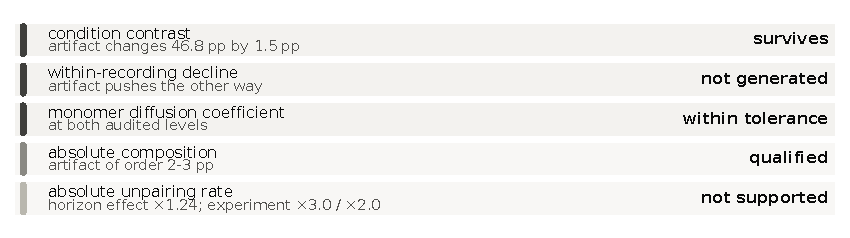
\includegraphics[width=\linewidth]{figures/fig3_payoff}
\caption{Grading each claim against the measured horizon effect. Because the audit gives the
effect's size and sign under the simulator, it permits a claim-specific sensitivity assessment.
Verdicts are carried by the words rather than by color, since blue and orange denote the two arms
throughout this paper. Simulator-to-experiment transfer is uncalibrated, so the effect serves as
a sensitivity scale rather than as a correction to any measurement.}
\label{fig:payoff}
\end{figure}

Using the same log-linear summary across window positions, the simulated
horizon effect increases the inferred unbinding rate by a factor of
approximately $\times1.24$ across a recording, compared with experimental
increases of approximately $\times3.0$ for MET-FAB and $\times2.0$ for
MET-INLB. This comparison establishes relative scale only; it neither
identifies the cause of the experimental trends nor supports interpreting a
whole-recording estimate as one constant unbinding rate.

\section{The census contrast}
\label{app:census}

\paragraph{Background for readers outside receptor biology.} MET is a receptor
tyrosine kinase of the plasma membrane. Its activation by hepatocyte growth
factor, or by the \emph{Listeria monocytogenes} surface protein InlB, is
associated with receptor dimerization and downstream signaling
\citep{dietz2013single,baldering2021crispr}. In single-particle tracking, individual receptors carry a fluorescent label
and are imaged at video rate in living cells; fluorescent spots are detected
and linked across frames to reconstruct trajectories and estimate receptor
mobility \citep{harwardt2017membrane}. The recordings used here
label MET either with a non-activating Fab fragment (resting condition) or
with fluorescent InlB (activated condition), 25 cells each. The estimator
reads every video as a realization of the simulated
$A + A \rightleftharpoons B \rightleftharpoons C$ model, so the inferred
composition is a model-conditional quantity, not a stoichiometric count.

\begin{figure}[h]
\centering
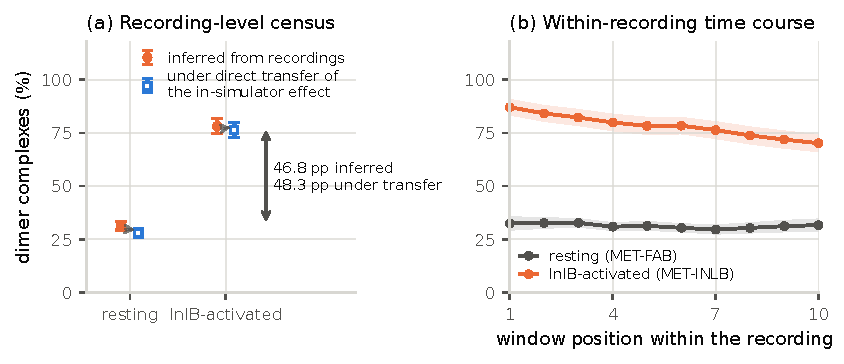
\includegraphics[width=\linewidth]{figures/figS1_census}
\caption{Inference results from experimental MET recordings
(Sec.~\ref{sec:census}). (a) The
model-conditional census of dimer complexes on MET single-particle-tracking
video, as inferred and under direct transfer of the in-simulator horizon
effect. The transferred effect lowers both conditions, the resting one
slightly more, so the contrast changes by only $1.5\pp$. This is a
sensitivity calculation: simulator-to-experiment transfer is uncalibrated, so
these are not corrected experimental estimates. Direct-transfer values
subtract the recording-level signed shift of simulated settings with initial
$\fD<0.4$ (resting-like, $n=115$) or $\fD>0.7$ (activated-like, $n=276$).
(b) The inferred dimer-complex fraction by window position, averaged over the
25 cells of each condition (band: cell-level s.e.m.); the activated
condition declines from $87.0\%$ to $70.2\%$ while the resting condition
remains near $31\%$. Only experimental inferences are drawn; in simulation, inherited
history shifts late windows upward ($+3.5\pp$ at window 10 for
activated-like settings), so it does not generate this decline. All error
bars and bands are cell-level standard errors; they do not represent
uncertainty in the transfer.}
\label{fig:census}
\end{figure}

Direct transfer changes the absolute composition estimates from $31.4\%$
and $78.2\%$ to approximately $28\%$ and $76\%$, respectively. These values
illustrate sensitivity to the simulated horizon effect and are not corrected
experimental estimates.

The transfer subsets are defined by the initial composition label of each
setting ($\fD<0.4$: $n=115$; $\fD>0.7$: $n=276$ of 500 settings), whereas
the strata of Appendix~\ref{app:strata} are defined by the true composition at
the window-10 start; the two groupings answer different questions. Grouped by
initial composition, the signed window-10 shift of $\fD$ is upward in both
subsets, $+5.6\pp$ $[4.1,7.2]$ for resting-like and $+3.5\pp$ $[2.0,5.1]$
for activated-like settings, and the recording-level means used for the
transfer are $+3.4\pp$ $[2.6,4.3]$ and $+1.9\pp$ $[0.7,3.0]$ (95\%
bootstrap intervals over settings). The negative window-10 shifts of the two
higher strata in Appendix~\ref{app:strata} describe the smaller group of
settings that still hold a mid or high composition at window 10. The
statement in Sec.~\ref{sec:census} that inherited history shifts late-window
$\fD$ upward therefore holds for the activated-like subset on which the
within-recording comparison relies, and the transfer remains a sensitivity
calculation for that selected scenario rather than a bound on experimental
bias.

\section{Truth reference and reproducibility}
\label{app:truthref}

This appendix documents how the cohort was completed and seeded, and why the
window-start population is the truth reference for $\fD$. Sampling continued
until 500 settings were completed. Two of 502 attempted
settings exceeded the available rendering memory and remain documented as
rejected draws. The analyzed cohort is therefore sampled from the training
prior conditional on renderability.

A persisted master seed deterministically generates one seed for every
(setting, arm, replicate) combination. Each result file also carries a cohort
digest, which the analysis verifies before use to prevent results from
different cohorts being mixed.

The estimator's training labels are window-start populations, so the window
start is the primary truth reference for $\fD$. The table reports descriptive
mean absolute error across 500 settings and ten clips or windows per setting in
each arm. Confidence intervals elsewhere resample matched settings, not the
correlated windows. Evaluating the same estimates against the
within-window mean asks about time-averaged composition rather than the
start-state estimand used for training. Under that alternative definition, the reset-arm error is $27\pp$ rather
than $2.9\pp$; this difference reflects a changed estimand, not a failure of
the estimator on its training target.

\paragraph{Interval widths.} The coverage decline of Sec.~\ref{sec:headline}
is not accompanied by wider intervals. From the saved posterior draws of all
500 settings, the mean width of the central 90\% interval for $\fD$ is
$15.1\pp$ $[14.5,15.8]$ at window 1 and $13.6\pp$ $[12.8,14.4]$ at window 10
in the continuous arm, against $15.2\pp$ $[14.5,15.9]$ for the reset clips
(95\% bootstrap intervals over settings); the paired change from window 1 to
window 10 is $-1.5\pp$ $[-2.1,-0.9]$. The central 50\% interval narrows
from $6.1\pp$ to $5.5\pp$ over the same windows, with $6.1\pp$ for the reset
clips. The intervals therefore narrow slightly while coverage falls from
$0.95$ to $0.39$.

\begin{table}[h]
\centering
\small
\begin{tabular}{lcc}
\toprule
truth reference for $\fD$ & reset arm & continuous arm (all windows) \\
\midrule
window start (primary) & $2.93\pp$ & $6.33\pp$ \\
window mean (sensitivity) & $27.00\pp$ & $9.00\pp$ \\
window end (sensitivity) & n/a & $10.34\pp$ \\
unrounded parameter label (sensitivity, resets only) & $2.89\pp$ & n/a \\
\bottomrule
\end{tabular}
\end{table}

\section{Estimator training and data splits}
\label{app:training}

The estimator audited in this study was trained once and then held fixed; we
did not retrain or tune it for either audit arm or for the experimental
recordings. All videos in these three datasets were independently generated
2\,s grayscale clips with 100 frames of $256\times256$ pixels.
Three physically separate datasets had distinct roles: 200,000 TRAIN videos
supplied gradient updates, 50,000 TEST videos supplied the per-epoch
model-selection loss, and 10,000 EVAL videos were used only for final
held-out recovery and for setting the audit tolerances reported in
Sec.~\ref{sec:system}. No video was shared among these datasets. The
tolerances were computed from the recovery's optimized point estimates
(Appendix~\ref{app:compute}); summarizing the same 10,000 videos by marginal
posterior medians gives log-scale mean absolute errors of $0.0222$ dex
($\times1.053$) for $\DA$ and $0.1788$ dex ($\times1.509$) for $\koff$,
against $0.0227$ dex ($\times1.054$) and $0.1773$ dex ($\times1.504$) from
the optimized estimates; using either recovery error as the tolerance leaves
the primary audit verdicts unchanged. The $\fD$ tolerance of $2.8\pp$ is composed from the count
medians. Table~\ref{tab:config} lists the prior ranges and the fixed
simulation and imaging settings behind every video in this study.

\begin{table}[h]
\caption{Configuration of the simulator, the imaging model, and the prior.
Priors are log-uniform between the stated bounds. The six emitter values are
the calibrated vector of the training corpus (the sample geometric median of
imaging estimates on the resting MET recordings), fixed for every training
video and for both audit arms. The five camera values were marginalized in
training: each training video drew them from the narrow log-uniform boxes
given in brackets, and both audit arms fixed them at the listed reference
values, which are the acquisition configuration for gain, baseline, and
quantum efficiency, the camera datasheet for read noise, and the median
photon offset measured on the MET recordings for the optical background.}
\label{tab:config}
\centering
\footnotesize
\setlength{\tabcolsep}{4pt}
\begin{tabular}{llp{0.46\linewidth}}
\toprule
group & quantity & value \\
\midrule
prior & initial counts $A_0$, $B_0$, $C_0$ & 1 to 316 each \\
 & monomer diffusion coefficient $\DA$ & 0.056 to 0.56\,\textmu m$^2$/s \\
 & relative mobility $D_B/\DA$, $D_C/\DA$ & 0.24 to 0.75; 0.01 to 0.10 \\
 & association efficiency $R_{\mathrm{ON}}$ & 0.01 to 1 \\
 & unbinding, immobilization, remobilization rates & 0.1 to 10\,s$^{-1}$ each \\
\midrule
simulation & field of view & $256\times256$ pixels of 158\,nm (40.4\,\textmu m square) \\
 & box depth; boundaries & 2\,nm (periodic); open in the plane \\
 & particle diameter (contact distance) & 10\,nm \\
 & frame interval; integration step & 0.02\,s (50 frames/s); 2\,ms (10 steps per frame) \\
 & frames per 2\,s clip; per 20\,s trajectory & 100; 1,000 \\
\midrule
emitter & PSF width, median $\sqrt{2}\sigma$ & 1.69 pixels (log-normal spread 0.18) \\
 & label brightness, median & 251 photons per frame (log-normal spread 0.67) \\
 & brightness flicker rate; bleaching & 3.39\,s$^{-1}$; probability 0.107 per 100 frames \\
 & dimer & two independent labels, photons added \\
\midrule
camera & gain & 41.8 ADU per photoelectron [41.7 to 42.2] \\
 & quantum efficiency & 0.90 [0.89 to 0.91] \\
 & optical background & 28.7 photons per pixel and frame [28.5 to 29.2] \\
 & baseline; read noise & 175 ADU [174 to 178]; 10.5 ADU [10.5 to 10.6] \\
 & storage & 8-bit integers, fixed range \\
\bottomrule
\end{tabular}
\end{table}

Training minimized the mean negative conditional log density of the true
log-transformed parameter vector for 50 epochs. We used AdamW with a minibatch
of 32 videos per process, an initial learning rate of $1.28\times10^{-3}$,
and the PyTorch 2.9.1 defaults $\beta_1=0.9$, $\beta_2=0.999$,
$\epsilon=10^{-8}$, and weight decay $0.01$. A
\texttt{ReduceLROnPlateau} scheduler monitored TEST loss with reduction factor
$0.5$, patience one epoch, absolute improvement threshold $10^{-4}$, and
minimum learning rate $10^{-5}$. After two non-improving epochs at the floor, the
enabled restart rule restored the best checkpoint and reduced the preceding
peak learning rate by a factor of four; restarts ended when the next peak
would not exceed the floor. The retained checkpoint was the epoch with the
lowest TEST loss; its mean loss was $-7.4801$.

TRAIN videos were augmented on loading by a uniformly sampled multiple of a
$90^\circ$ rotation and independent horizontal and vertical flips, each with
probability $0.5$; augmentation was disabled for TEST and EVAL. Integer video
values were scaled to $[0,1]$, and parameter targets were transformed to base-10
logarithms. The conditional masked autoregressive flow contained five
autoregressive transforms, each with two residual blocks and 50 hidden
features. It used structured standardization of parameter targets and
conditioning videos, batch normalization, and dropout probability $0.1$.
TRAIN/TEST/EVAL generation and estimator training did not impose a fixed random seed;
the generated datasets and retained estimator were persisted. The code at
the version used for this study, the persisted results behind every figure
and table, and the scripts that regenerate them are released at
\url{\repourl}; the video corpora are not bundled, and the repository states
what can be reproduced from the included materials.

\newpage
\section{Computational resources}
\label{app:compute}

Computational resources for the reported study and the wider project
included the Goethe-NHR cluster at Goethe University Frankfurt, the JUWELS and
JUPITER systems at the J\"ulich Supercomputing Centre, and local
workstations. The descriptions below distinguish resources used for the
reported study from those used elsewhere in the project. We distinguish
measured wall times from scheduler allocations and linear projections. Wall
times exclude queueing; the CPU and GPU systems were managed with Slurm.

\paragraph{Synthetic corpus generation.} The 2\,s biological-state corpus
contained 200,000 TRAIN, 50,000 TEST, and 25,000 EVAL videos; 10,000 of the
EVAL videos were used for the recovery analysis in this paper. Generation used
28 single-node CPU-array elements (20 TRAIN, five TEST, and three EVAL). Each
node ran at most ten independent generation processes with four x86-64 CPU
cores and 17.6\,GB of requested memory per process, for 40 cores and 176\,GB
per node. At most 40 nodes were allowed to run concurrently. Each node had an
18\,h wall-time allocation, giving an upper allocation budget of 504 node-hours
(20,160 core-hours); actual jobs generally ended before that limit. The
TRAIN+TEST videos occupy 662.4\,GiB.

\paragraph{Estimator training and held-out recovery.} A measured timing
reference for the same 2\,s estimator pipeline used an exclusive node with
four AMD Instinct MI210 GPUs (64\,GB each), 64 data-loading workers, 480\,GB
of host memory, and networked scratch storage. With 50,000 TRAIN and 10,000
TEST videos and batch size 32 per process, ten epochs took 13,246\,s
(3.68\,h); steady epochs took approximately 1,267\,s. Scaling this measured
rate by the number of videos per epoch gives a simple linear reproduction
estimate of approximately 74 node-hours, or 296 GPU-hours, for the
200,000/50,000-video, 50-epoch training reported here. This is a workload
projection rather than the retained run's wall time. The final held-out
recovery was measured directly: 10,000 EVAL videos, sharded evenly over eight
MI210 GPUs on a 64-CPU-core, 480\,GB node, completed in 4,781\,s (1.33\,h;
10.6 GPU-hours). Each recovery used 1,000 optimization steps.

\paragraph{Horizon audit.} Audit generation ran on a 62\,GB x86-64 host. Up
to six settings were generated concurrently for typical draws, while dense
settings were serialized. A completed setting, comprising one 20\,s
trajectory and ten independent 2\,s resets, took 79--833\,s to generate;
dense completed settings used approximately 25--35\,GB of memory. Two
high-reaction-traffic draws exceeded 128\,GB and could not be rendered on this
host. They remain documented as rejected draws, and the cohort was completed by
continuing to sample from the same prior. Processing the 500-setting cohort in batches of
100 limited temporary video storage to approximately 5\,GB. Posterior sampling
for the resulting 10,000 windows used one NVIDIA RTX 6000 Ada GPU (48\,GB) and
1,000 posterior draws per window; pilot timings imply approximately 1.25 GPU-hours
for the complete cohort. The latter is a scaled timing estimate because the
aggregate inference wall time was not retained.

\paragraph{Compute outside the reported experiment.} The wider two-stage
project generated a second, separate 275,000-video corpus for imaging-parameter
inference, for approximately 550,000 synthetic videos across both stages. It
also used four-GPU NVIDIA GH200 nodes for other GPU-heavy analyses. Those costs
are not included in the audit totals above.

\end{document}
